\section{Model architecture}
\label{section:Architecture:Model}

We propose a prediction framework based on the one presented in \cite{Zhao2019}.
Creating a Convolutional autoencoder and LSTM method for time series prediction should provide some benefits.
Primarily, the combination of methods should help with increasing the prediction accuracy in data with high fluctuations.
Unlike the univariate method used in \cite{Zhao2019} we intend to improve upon the method by applying it as a global method and a multivariate method.
Such a method has never been explored in the E-commerce forecasting domain, warranting the exploration of the method's applicability to the problem space.
% Add explainer to why we do this?
% Add line as to explain that this is a new method in E-commerce forecasting?

The proposed framework is comprised of two parts: the convolutional autoencoder and the LSTM.

The convolutional autoencoder process the input data, extracting a feature set by deconstructing the data.
This is done through the encoder. After this, the decoder is used to reconstruct the input data.
By doing this, the noise in the input data should be decreased to some extent.

The second part of the architecture is the LSTM module.
This module is intended to extract the temporal features of the dataset
in order to predict future values in the time series.

\begin{figure}[h!]
    \centering
    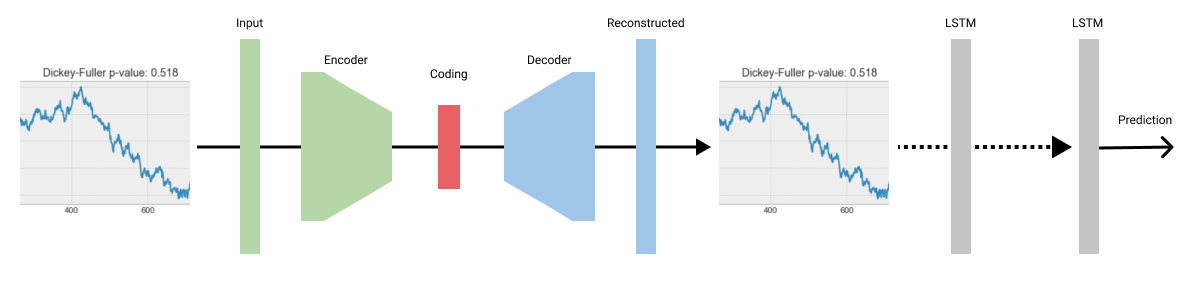
\includegraphics[width=\textwidth]{./sections/Architecture/figures/CNN-AE + LSTM.png}
    \hfill
    \caption{Illustration of a CNN-AE + LSTM network.}
    \label{fig:stacked_autoencoder_arch}
\end{figure}

Finally, the complete framework proposed in this paper connects these two models,
creating a convolutional autoencoder and LSTM framework for making predictions.
These predictions are intended to function on time series data with high fluctuations,
making accurate and less error-prone predictions than simple statistical or deep learning methods.


As a means to validate the proposed method, predictive benchmarks should be provided.
Established methods such as the SARIMA method and the LSTM method are well suited for this.
These methods create a baseline that can be used to establish the comparative performance with the proposed method.

The motivation behind the proposed framework is explored in further detail later in section \ref{section:Discussion}.

